%%%%%%%%%%%%%%%%%%%%%%%%%%%%%%%%%%%%%%%%%%%%%%%%%%%%%%%%%
%                 File: UV1310cdc.tex               	%
%                  Date: 10 Oct, 2015                	%
%                                                    	%
%   For submission to a OFC      						%
%                                                     	%
%   Technical paper about the results obtained with   	%
%   professor Wei Shi with tunable cascaded				%
%	contra-directional coupler				      		%
%	+ theorical analysis								%
%%%%%%%%%%%%%%%%%%%%%%%%%%%%%%%%%%%%%%%%%%%%%%%%%%%%%%%%%



\documentclass[letterpaper,10pt]{article}
\usepackage{osameet2}

\usepackage[utf8]{inputenc} %encoding of the input(this text file)
\usepackage[T1]{fontenc} 	%uses the right font encoding
\usepackage{lmodern,textcomp}		%makes font work for fontenc
\usepackage[french,english]{babel} %multiple languages
\selectlanguage{english}	%can switch to french later using this

\usepackage{ulem}
\usepackage{amsmath,amssymb}

\usepackage{graphicx,epsfig,epstopdf}

\usepackage{xcolor}
\newcommand\todo[1]{\textcolor{red}{#1}}
%\renewcommand\todo[1]{}  %activate to get rid of comments

\begin{document}

\title{O-band Silicon Photonic Bragg-Grating multiplexers using UV lithograpy}
%\title{Apodized O-band contra-directional coupler fabricated using UV lithography}



\author{Jonathan St-Yves, Sophie Larochelle, and Wei Shi$^*$}
\address{Centre d'optique, photonique et laser (COPL) and Département de génie électrique, Université Laval, 2375 rue de la Terrasse, Québec (Québec), Canada, G1V 0A6}
%\email{jonathan.st-yves.1@ulaval.ca}
\email{$^*$wei.shi@gel.ulaval.ca}

\ocis{ (130.7408) Wavelength filtering devices; (350.2770) Gratings; (130.3120)   Integrated optics devices}


\begin{abstract}
We demonstrate 4 channel Bragg-grating based WDM fabricated using 193 nm lithography on the silicon on insulator platform with small features under 140 nm for use in the O-band.
\end{abstract}



\maketitle


\section{Introduction}
\subsection{Relevance and place in the greater scheme}
\todo{Point out that optical filters are needed for WDM. }

\subsection{State of the Art}
\todo{Speak about lattice filters, echelle/arrayed waveguides, ring on SOI. None of these are flat top, limited FSR, low bandwidth. Bragg gratings only reflect. Apodized contra-DC only work on E-beam.}

Integrated WDM is currently achieved using lattice filters\cite{horst2013cascaded} or arrayed waveguides \cite{okamoto2013fabrication}, though these methods use a large footprint and have a limited free-spectral range. Others possible approaches include Bragg gratings\cite{simard2012apodized} and micro-ring filter\cite{xu2006cascaded}.

\subsection{Challenges}
\todo{Small corrugation size and period, expecially at 1310. Accuracy for apodization. Large enough coupling}
Contra-directional couplers can offer large bandwidth, compact footprint and high sidelobes suppression, but the small feature size needed for gratings limits the performance when fabricated with conventional deep-ultraviolet lithography\cite{shi2013ultra}\cite{shi2013coupler}. This issue is compounded when designing a device for the O-band (around 1310 nm), which is an useful band for lower dispersion in conventional fibers and additional bandwidth, as the small wavelength size requires a proportionally smaller grating step.



\section{Device}
\subsection{Design} 
\todo{Slab and thin waveguides for bigger overlap. Traditional apodized side-wall grating.}
\begin{figure}[htbp]
	\centering
	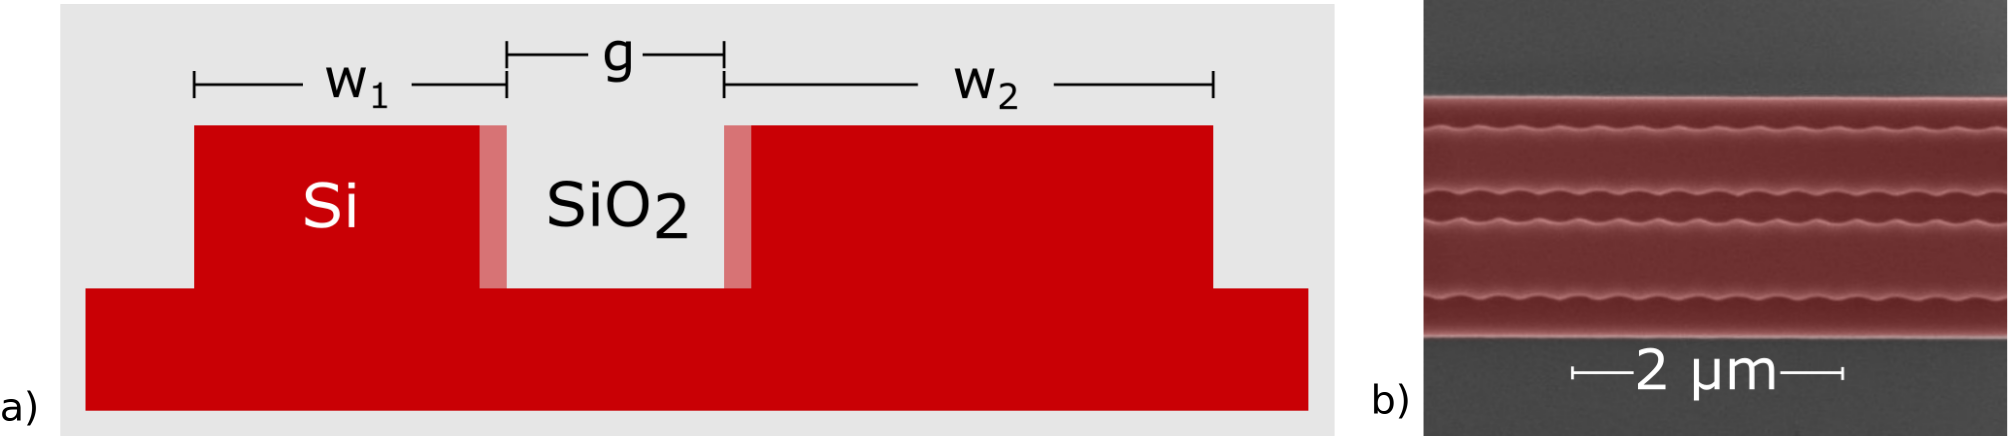
\includegraphics[width=.99\columnwidth]{CrossAndTop}
	\caption{ (a)Schematic cross-section: The contra-directional coupler is made of two silicon waveguides of different widths $w_1$ and $w_2$ with an average gap $g$ in-between them. The gap varies along the propagation axis. (b) Colored microscope top view of the grating shows the shape of the corrugations after fabrication with ultraviolet lithography. }
	\label{fig:Device}
\end{figure}
Figure \ref{fig:Device} shows the proposed structure.

The contra-directional coupler consists of two waveguides in close proximity, with a periodic change to the gap in-between them. This causes a wavelength selective contra-directional coupling at  $\lambda_\text{c} = \Lambda (n_\text{1}+n_\text{2})$, where $\Lambda$ is the grating pitch, and $n_\text{1}$ and $n_\text{2}$ are the effective refractive indices of the first-order and second-order eigenmodes in the coupler. 
The waveguides are highly asymmetric to suppress the co-directional coupling that would occur with two identical waveguides.

\subsection{Fabrication process}
\todo{Fabrication using a CMOS compatible UV lithography with a phase-shifted mask.}

\subsection{Fabrication result}
\todo{Clear corrugations and the possibility to have a small gap under 140 nm.}
\begin{figure}[htbp]
	\centering
	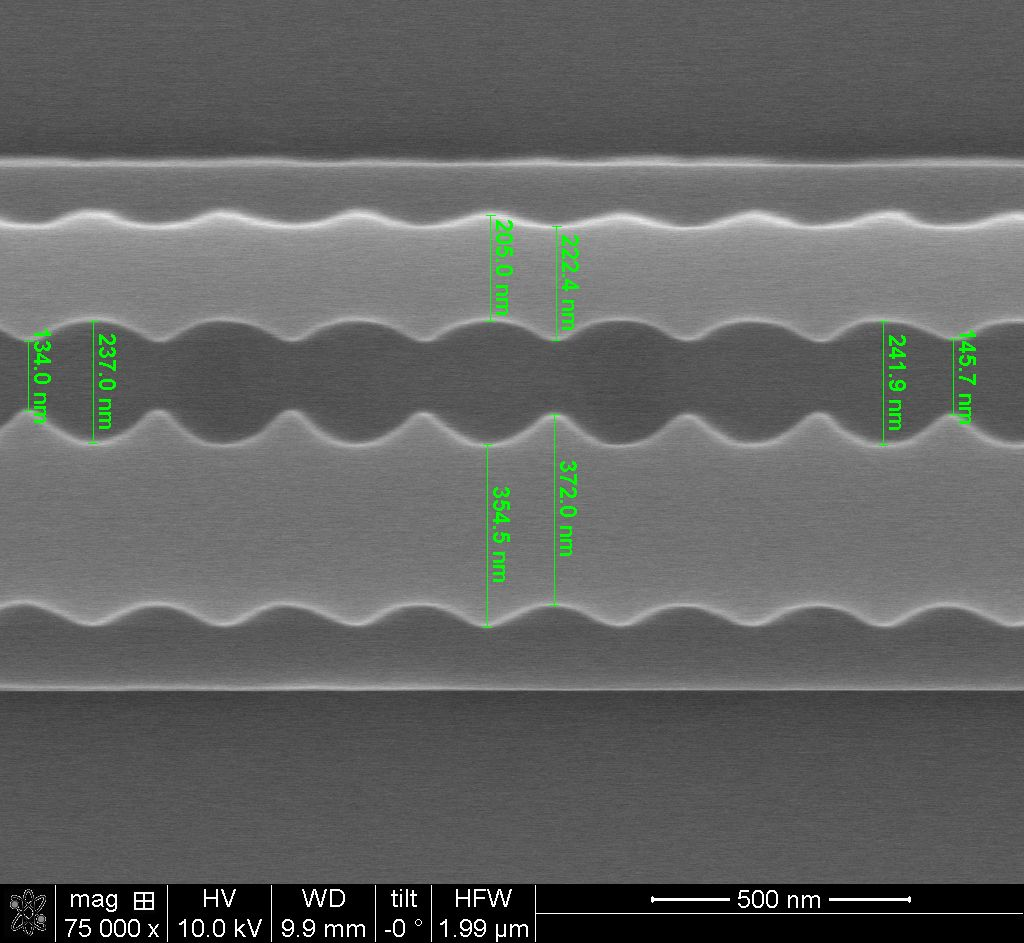
\includegraphics[width=.60\columnwidth]{1310_P36_g190maybe}
	\caption{SEM picture of a strong grating. The measurements show that the widths of the waveguides are not the same in the close and far region, resulting in a strong change of index along the propagation direction and a distortion of the apodization profile. }
	\label{fig:litho}
\end{figure}

\subsection{Filter optical performance}
\todo{[Plot of the optical response ]}

\subsection{WDM performance}
We see in figure \ref{fig:WDM} the response of the filter using a single filtering stage and also for two filtering stages.
\begin{figure}[htbp]
	\centering
	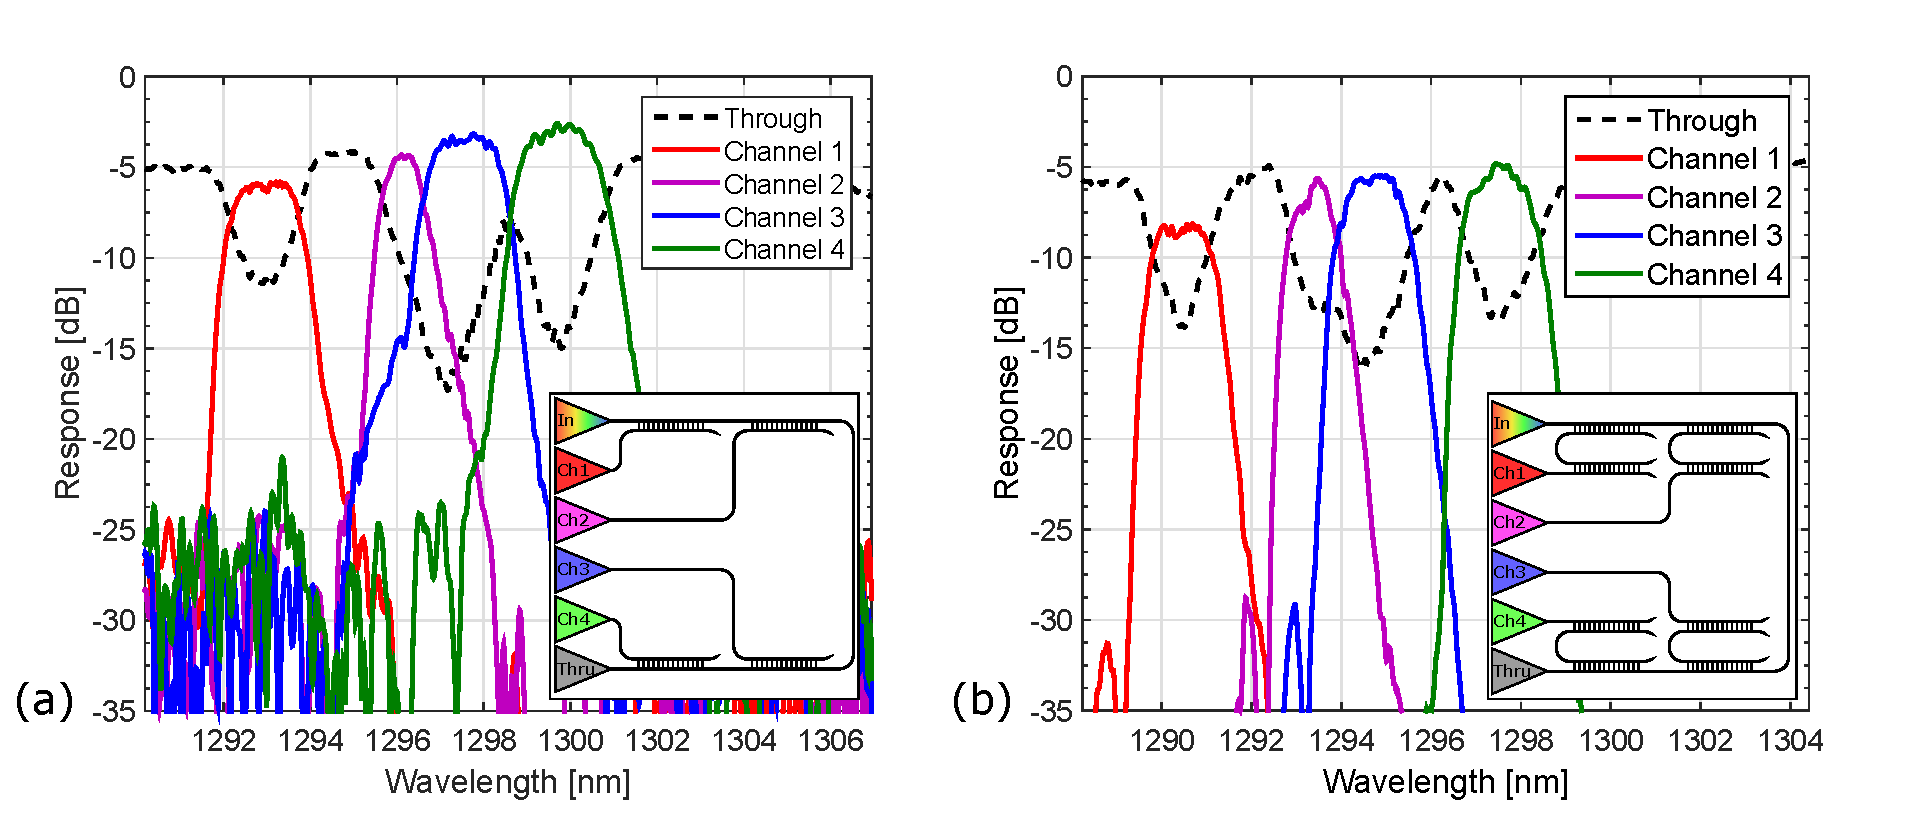
\includegraphics[width=.99\columnwidth]{WDM}
	\caption{a) Single stage WDM. b) Double staged WDM }
	\label{fig:WDM}
\end{figure}




\section{Conclusion}
\todo{The demonstrated device open possibilities for wide bandwidth and temperature tolerant filters with a flat top response. Next prototypes promise to offer even larger bandwidth and a more square shape after biasing for lithography.}













\section*{Acknowledgments}
We acknowledge CMC Microsystems for the  software and the fabrication subsidy. The authors acknowledge the Natural Sciences and Engineering Research Council of Canada for funding this research. This work is part of the SPEED research project (Silicon Photonic Electrically Engineered Devices) funded by NSERC (RDCPJ438811-12), PROMPT (PJT-2011-17), and TeraXion.

\bibliographystyle{osajnl}
\bibliography{bibli}

\end{document}